\chapter{Tecnologie}
\section{PowerPlatform}
PowerPlatform è una piattaforma Microsoft che racchiude vari strumenti per agevolare l’organizzazione usando strumenti innovativi e basati sul principio low-code.
Offre tantissimi modelli di qualsiasi tipologia da cui partire per creare ciò che si desidera.
Inoltre si ha molta scelta per caricare i dati sia da altri strumenti Microsoft sia da servizi esterni o anche da origini locali. \newline
Power Platform offre i seguenti software, alcuni solo online altri anche in versione dsektop dove permettono maggiori personalizzazioni.\\
Per l'illustrazione dei loghi della piattaforma si veda la \figurename \space \ref*{fig:PowerPlatform}.
\begin{figure}[H]
    \centering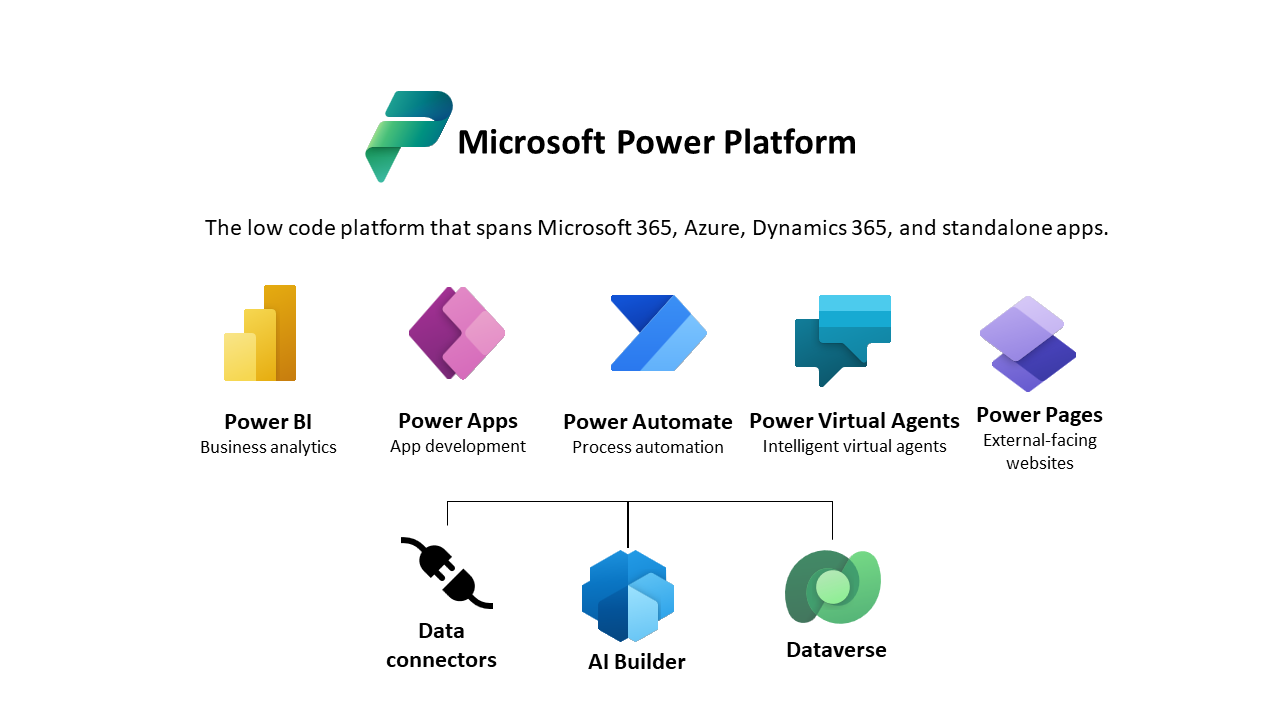
\includegraphics[width=\textwidth, height=\textheight,keepaspectratio]{immagini/Icone-PowerPlatform.png}
    \caption{Loghi PowerPlatform}
    \label{fig:PowerPlatform}
\end{figure}
\begin{description}
    \item \textbf{Power Bi:} permette l’analisi in autonomia di molti dati con parecchi strumenti per personalizzare la gestione e la visualizzazione anche mediante le funzionalità di intelligenza artificiale.
    \item \textbf{Power Apps:} permette di creare rapidamente applicazioni da zero o da modelli, il codice è necessario solo per impostare le proprietà degli elementi aggiunti.
    \item \textbf{Power Automate:} permette di automatizzare i processi organizzativi tramite l’impostazione di flussi che si attivano al seguito di un evento o in maniera ricorrente.
    \item \textbf{Power Virtual Agents:} permette di creare velocemente dei chatbot basati sull’intelligenza artificiale con anche la possibilità di usare più lingue.
    \item \textbf{Power Pages:} permette di creare rapidamente siti web, offre la possibilità di raccogliere i dati dei visitatori mediante Microsoft Dataverse.
\end{description}

\section{Sharepoint}
Sharepoint è una piattaforma di collaborazione, sviluppata da Microsoft, che permette di creare \glossario{intranet} tra membri dello stessa divisione, progetto agevolando la condivisione di materiale, la comunicazione, la creazione di applicazioni, siti personalizzati e liste condivise.
Inoltre permette molta personalizzazione anche per la tipologia di accesso ad ogni elemento per ogni membro; per il logo si veda la \figurename \space \ref*{fig:SharePoint}. 
In particolare SharePoint offre la possibilità di creare e condividere liste mediante il software Microsoft Lists.
\begin{figure}[H]
    \centering
\includegraphics[width=0.3\textwidth, height=0.3\textheight,keepaspectratio]{immagini/logo-Sharepoint.png}
    \caption{Logo SharePoint}
    \label{fig:SharePoint}
\end{figure}

\begin{description}
    \item \textbf{Microsoft Lists} è un servizio molto semplice e intuitivo con cui poter creare una lista di record in cui si può scegliere se visualizzare le colonne già previste di default o aggiungere nuove colonne specificando anche la tipologia di dato che verrà inserito. Per il logo si veda la \figurename \space \ref*{fig:M-Lists}.
\end{description}
\begin{figure}[H]
    \centering
\includegraphics[width=0.3\textwidth, height=0.3\textheight,keepaspectratio]{immagini/logo-MicrosoftLists.png}
    \caption{Logo Microsoft Lists}
    \label{fig:M-Lists}
\end{figure}

\section{Applicazione per gli operatori del magazzino}
Power Apps è lo strumento di PowerPlatform utilizzato in questa applicazione.
\subsection{DB2}
DB2 è un Relational Database Management System della IBM che permette di archiviare, gestire una grande mole di dati garantendo elevate prestazioni ed alta affidabilità con transazioni a bassa latenza.
Si utilizzano i comandi SQL\textsuperscript{1} per interrogare il database; per il logo si veda la \figurename \space \ref*{fig:DB2}.
\begin{figure}[H]
    \centering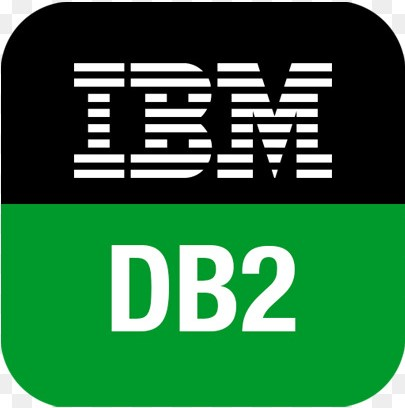
\includegraphics[width=0.3\textwidth, height=0.3\textheight,keepaspectratio]{immagini/logo-ibm-db2.jpg}
    \caption{Logo DB2}
    \label{fig:DB2}
\end{figure}

\subsection{Microsoft SQL}
Microsoft SQL Server, prodotto da Microsoft, è uno dei RDBMS\footnote{Relation Database Management System} più diffusi al mondo. 
Utilizza una variante del linguaggio SQL\footnote{Structured Query Language} standard, Transact-SQL sviluppato da Microsoft stesso; per il logo si veda la \figurename \space \ref*{fig:M-SQL}.
\begin{figure}[H]
    \centering
\includegraphics[width=0.3\textwidth, height=0.3\textheight,keepaspectratio]{immagini/logo-SqlServer.png}
    \caption{Logo Microsoft Sql Server}
    \label{fig:M-SQL}
\end{figure}


\section{Applicazione per il personale IT}
Power Apps, Power Automate e Power Bi compresa la versione desktop sono i software di PowerPlatform utilizzati per questa applicazione; inoltre viene utilizzata Microsoft Lists che viene salvata su un sito SharePoint.

\section{Applicazione per l'inserimento richieste ordini}
Power Apps, Power Automate sono i software di PowerPlatform utilizzati per questa applicazione; inoltre viene utilizzata Microsoft Lists che viene salvata su un sito SharePoint.
